\subsection{Pensando separadamente}
O problema clássico tem o potencial
\begin{equation}
    V(\vet q) = - G \sum_{a < b} \dfrac{m_a m_b}{r_{ab}},
\end{equation}
que é uma função homogênea com grau -1, ou seja, sendo $k \in \R$, temos
\begin{equation}
    V(k \vet q) = |k|^{-1} V(\vet q).
\end{equation}
Também vale observar que a energia cinética $T$ é uma função homogênea de grau 2, pois $T(k \vet p) = k^2 T(\vet p)$. Com isso, se quisermos obter uma determinada energia $\tilde E$, podemos buscar $\tilde{\vet q_a} = \alpha^{-1} \vet q_a$ e $\tilde{\vet p_a} = \beta \vet p_a$ de modo que
\begin{equation}
    T(\tilde{\vet p_a}) + V(\tilde{\vet q}) = \beta^2 T_0 + \alpha V_0 = \tilde E.
\end{equation}

Existem muitas formas de lidar com isso, sendo possível obter qualquer $\tilde E \geq 0$ apenas com $\beta$. No geral, podemos tomar, por exemplo,
\begin{equation}
    \alpha = 1 + \dfrac{\tilde E}{V_0},
    \quad
    \beta = \sqrt{-\dfrac{V_0}{T_0}}.
\end{equation}
Essa forma tem alguma vantagem? Não sei.

Já para o momento linear total, se queremos obter $\tilde P \in \R^3$ precisamos aplicar um tipo de "translação" nas velocidades, semelhante ao que pode ser feito para anular o centro de massas. Precisamos encontrar um vetor $\vet w_{\tilde P}$ tal que, definindo $\tilde{\vet p_a} = \vet p + m_a \vet w_{\tilde P}$, consigamos:
\begin{align}\label{eq:transformacao_momento_linear}
    \sum_{a=1}^N \tilde{\vet p_a} = \vet P_0 + M \vet w_{\tilde{\vet P}} = \tilde{\vet P} \
    \Rightarrow \ \vet w_{\tilde{\vet P}} = M^{-1} (\tilde{\vet P} - \vet P_0)
\end{align}

Para o momento angular, desenvolvemos independentemente uma forma de transformá-lo, mas que já constava em \cite[p.135]{aarseth_gravitational_2003} para um caso específico de 2 corpos.

De toda forma, existem diferenças na forma de tratar conforme a dimensão do problema. Se temos um conjunto de dados planar, o momento angular pode ser visto como um escalar, uma vez que $\vet J = (0, 0, J)$, então podemos buscar $\vet \omega = (0, 0, \omega)$ e definir $\tilde{\vet p_a} = \vet p_a + m_a \vet q_a \times \vet \omega$. Temos:
\begin{equation}
    \sum_{a=1}^N \vet q_a \times \tilde{\vet p_a}
    = \vet J_0 + \sum_{a=1}^N m_a \vet q_a \times (\vet q_a \times \vet \omega).
\end{equation}
Nesse caso bidimensional, $\vet q_a \times \vet \omega = \omega (-\vet q_a^{(2)}, \vet q_a^{(1)}, 0)$, e logo $\vet q_a \times (\vet q_a \times \vet \omega) = \vet \omega \norma{\vet q_a}^2$. Impondo a restrição:
\begin{equation}
    \vet \omega = \dfrac{1}{I_0}(\tilde{\vet J} - \vet J_0).
\end{equation}

\begin{figure}[H]
    \centering
    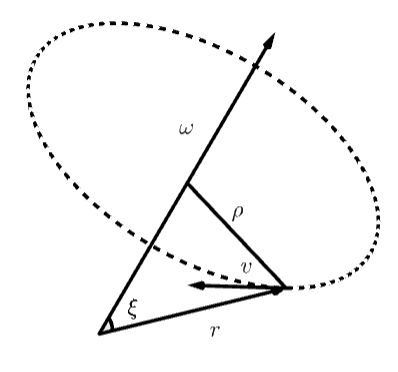
\includegraphics[width=0.3\linewidth]{img/rotacao.png}
    \caption{Representação de uma partícula e seu eixo de rotação.}
    \label{fig:angular_3d}
\end{figure}

No caso tridimensional a coisa é um pouco mais complicada. Considere uma partícula com posição $\vet r$ e um vetor $\vet \omega$ que define um eixo de rotação do qual $\vet r$ se distancia em $\rho$ e forma um ângulo $\xi$ e também cuja velocidade da partícula em relação a é $\vet v$, como na figura \ref{fig:angular_3d}. Nessa situação, temos que $\norma{\vet v} = \rho \norma{\vet \omega}$ e $\sin \xi = \rho / \norma{\vet r}$. Uma vez que $\vet v \perp \vet \omega$ e $\vet v \perp \vet v$, podemos concluir que $\vet v || \vet r \times \vet \omega$. Mais ainda, temos que:
\begin{equation}\label{eq:angular_def_omega}
    \norma{\vet r \times \vet \omega}
    = \norma{\vet r} \norma{\vet \omega} \sin \xi = \norma{\vet v}
    \Rightarrow
    \vet v = \vet r \times \vet \omega.
\end{equation}

O momento angular $\vet J$ também é um vetor perpendicular a $\vet r$ e a $\vet v$, mas $\vet J$ e $\vet \omega$ só são colineares quando $\vet r \perp \vet \omega$ (como no caso 2d). Apesar disso, a partir de (\ref{eq:angular_def_omega}) podemos construir um operador $\bm I: \R^3 \to \R^3$ em função de $m$ e $\vet r$ que leva $\vet \omega$ em $\vet J$. O operador tem a seguinte forma:
\begin{equation}
    \bm I = m
    \begin{bmatrix}
        - (r_2^2 + r_3^2) & r_1 r_2 & r_1 r_3 \\
        r_1 r_2 & - (r_1^2 + r_3^2) & r_2 r_3 \\
        r_1 r_3 & r_2 r_3 & - (r_1^2 + r_2^2)
    \end{bmatrix}.
\end{equation}
O operador $\bm I$ é denominado \textbf{tensor de inércia}, e muitas vezes aparece com o sinal oposto. Para facilitar, a partir daqui tomaremos $\bm W := \bm I$ sempre que um tensor de inércia for mencionado.

No caso de diversos corpos, a ideia é definir um eixo de rotação comum e a partir dele aplicar transformações sobre a velocidade angular de cada corpo. Seja $\bm I_T = \sum_{a=1}^N \vet q_a$ (ou seja, baseado somente nos valores pré-condicionamento). Para obter um momento angular desejado $\tilde{\vet J}$, basta encontrar um eixo $\vet \omega$ tal que $\bm I_T \vet \omega = \tilde{\vet J} - \vet J_0$ e aplicar a transformação 
\begin{equation}\label{eq:transformacao_momento_angular_3d}
    \tilde{\vet p_a} = \vet p_a + m_a \vet q_a \times \vet \omega.
\end{equation}

Diante do exposto, é evidente que as transformações propostas se sobrepõem. Por exemplo, no condicionamento da energia com $\tilde{\vet q} = \alpha^{-1} \vet q$ e $\tilde{\vet p} = \beta \vet p$, temos:
\begin{equation}
    \vet P(\tilde{\vet p}) = \beta \vet P_0,
    \quad
    \vet J(\tilde{\vet q}, \tilde{\vet p}) = \dfrac{\beta}{\alpha} \vet J_0.
\end{equation}

Além disso, qualquer "translação" nos momentos lineares, como feito em (\ref{eq:transformacao_momento_linear}) e (\ref{eq:transformacao_momento_angular_3d}), afeta fortemente a energia cinética do sistema, o que deve ser levado em conta na hora de condicionar um sistema por completo.
